\chapter{Implementacija i korisničko sučelje}
		
		
		\section{Korištene tehnologije i alati}
		
		Komunikacija u timu je ostvarena putem korištenja aplikacije WhatsApp\footnote{\url{https://www.whatsapp.com/}}. Komunikacija sa asistentom ostvarena je korištenjem aplikacije Microsoft Teams\footnote{\url{https://www.microsoft.com/hr-hr/microsoft-teams/group-chat-software/}}. Za izradu dijagrama korišten je Astah Professional\footnote{\url{https://astah.net/products/astah-professional/}}. Za upravljanje izvornim kodom korišten je alat Git\footnote{\url{https://git-scm.com/}}. Udaljeni repozitorij projekta nalazi se na platformi GitHub\footnote{\url{https://github.com/}}.
		
		Kao razvojno okruženje na backendu korišten je IntelliJ\footnote{\url{https://www.jetbrains.com/idea/}}, a na frontendu Visual Studio Code\footnote{\url{https://code.visualstudio.com/}}. Visual Studio Code je razvojno okruženje tvrtke Microsoft za Windows, Linux, macOS. Za razvoj softvera koristi Microsoftove platforme poput Windows API, Windows Forms, Windows Presentation Foundation, Windows Store i Microsoft Silverlight.
		
		Tehnologije korištene za razvoj backenda su Spring Boot\footnote{\url{https://spring.io/projects/spring-boot}} i programski jezik Java\footnote{\url{https://www.java.com/en/}}. Tehnologije korištene za razvoj frontenda su Angular\footnote{\url{https://angular.io/}} i programski jezik TypeScript\footnote{\url{https://www.typescriptlang.org/}}. Angular je besplatni okvir(framework) za izgradnju web aplikacija otvorenog izvornog koda temeljen na TypeScriptu. Angular se temelji na principu komponenata gdje nekoliko nezavisnih komponenti surađuje kako bi oblikovali korisničko sučelje. Takva struktura čini aplikacije lako prilagodljivim i održivim.
		
		Za automatizirano testiranje koristen je alat Selenium IDE\footnote{\url{https://www.selenium.dev/documentation/ide/}}. Za puštanje aplikacije u pogon korištena je platforma Render\footnote{\url{https://render.com/}}.
		
		Baza podataka zadužena za pohranu podataka je PostgreSQL\footnote{\url{https://www.postgresql.org/}}.
		
		
	
	
	
		\section{Ispitivanje programskog rješenja}
			
			\subsection{Ispitivanje komponenti}
			
			Ispitivanje komponenti ostvareno je pomoću Spring Boot i JUnit 5 alata za ispitivanje.
			
			Na slikama 5.1 i 5.2 prikazani su testovi vezani uz voditelja. Oba testa pokušavaju dodati voditelja na postaju. Na slici 5.1 prikazan je kod iz testa koji uspješno dodaje voditelja na postaju. Slika 5.2 prikazuje kod iz testa gdje se provjerava može li se dodati voditelj na nepostojeću postaju. Vraća da je uspješan test ako se ne može dodati što se i očekuje s ozbirom da je u pitanju nepostojeća postaja.  
			
			\begin{figure}[H]
				\centering
				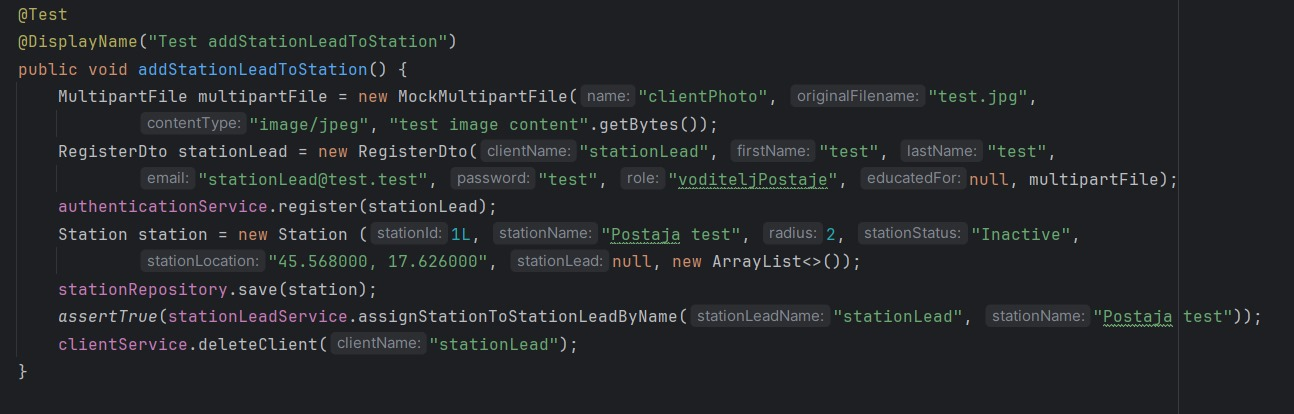
\includegraphics[width=\textwidth]{slike/voditelj1.JPEG}
				\caption{Testiranje za uspješno dodavanje voditelja postaji}
				\label{fig:dijagram_baze}
			\end{figure}
			
			\begin{figure}[H]
				\centering
				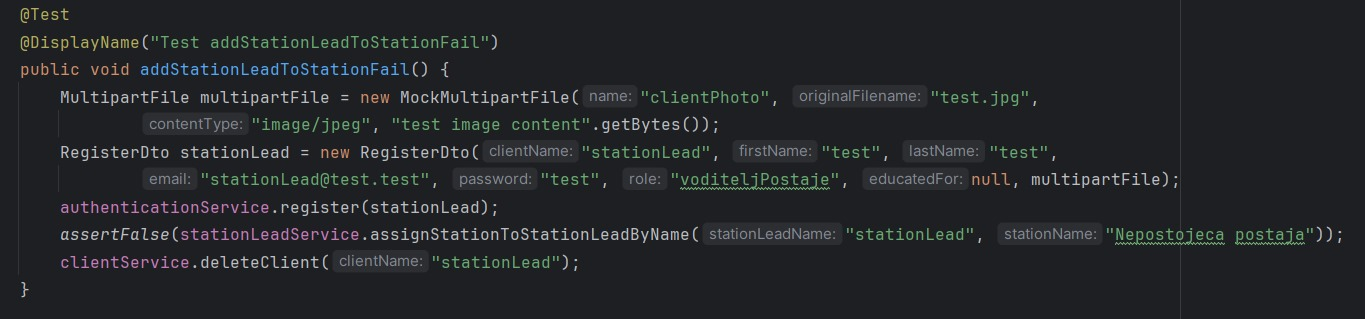
\includegraphics[width=\textwidth]{slike/voditelj2.JPEG}
				\caption{Testiranje za dodavanje voditelja nepostojećoj postaji}
				\label{fig:dijagram_baze}
			\end{figure}
			
			Sljedeća tri testa vezana su uz tragača. Prvi od njih nalazi se na slici 5.3 te provjerava jesu li se vozila dobro dodala na tragače pri registraciji. Sljedeći test čiji je kod prikazan na slici 5.4 dodaje tragača na postaju. Zatim provjerava je li postaja prazna? Test je uspješan ako vrati da nije prazna jer smo prethodno dodali tragača. Posljednji test vezan uz tragača miče tog tragača kojeg smo prethodno dodali iz postaje. Zatim provjerava je li postaja prazna? Ovaj put je test uspješan ako vrati da je postaja prazna. Kod je prikazan na slici 5.5. 
			
			\begin{figure}[H]
				\centering
				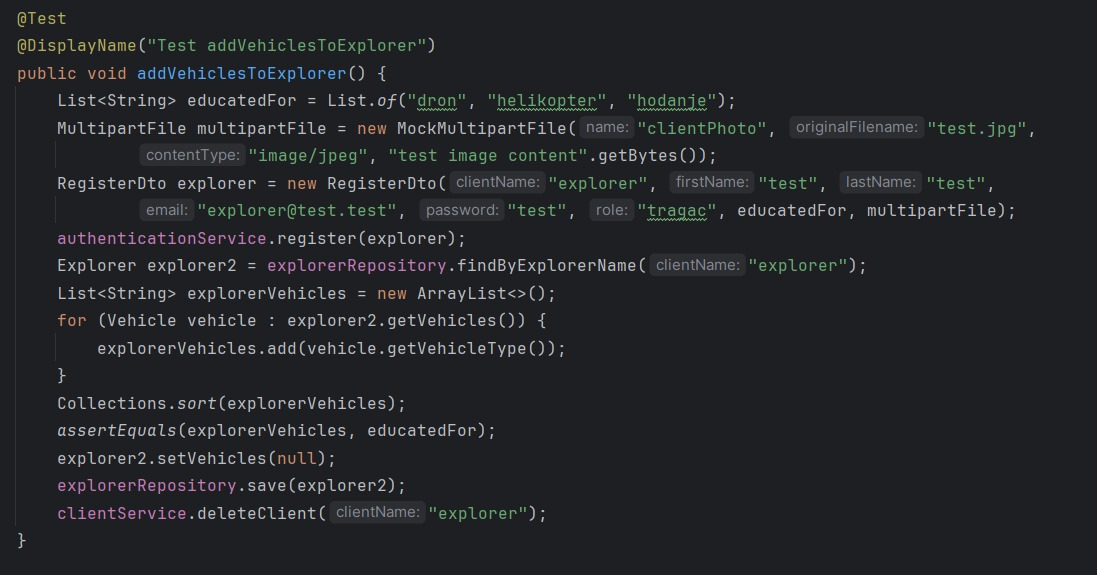
\includegraphics[width=\textwidth]{slike/tragac1.JPEG}
				\caption{Testiranje jesu li se vozila dodala na tragače}
				\label{fig:dijagram_baze}
			\end{figure}
			
			\begin{figure}[H]
				\centering
				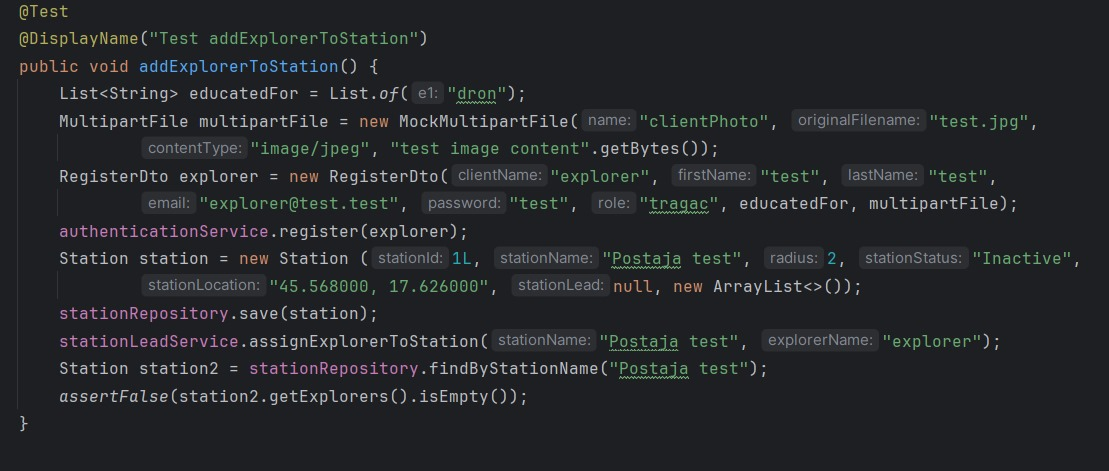
\includegraphics[width=\textwidth]{slike/tragac2.JPEG}
				\caption{Testiranje je li postaja prazna }
				\label{fig:dijagram_baze}
			\end{figure}
			
			\begin{figure}[H]
				\centering
				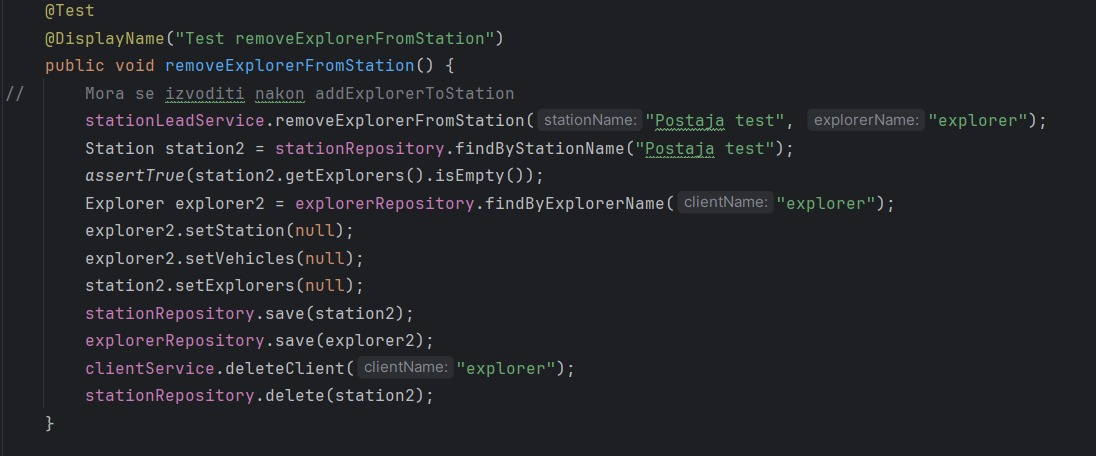
\includegraphics[width=\textwidth]{slike/tragac3.JPEG}
				\caption{Testiranje je li postaja prazna }
				\label{fig:dijagram_baze}
			\end{figure}
			
			Na slikama 5.6 i 5.7 prikazani su testovi vezani uz istraživača. Nakon što se korisnik registrira i zatraži ulogu istraživač potrebna je još dodatna potvrda od strane admina. Na slici 5.6 prikazan je test kod kojeg se prihvaća istraživač nakon registracije. U slučaju testa na slici 5.7 zahtjev je odbijen. 
			
			\begin{figure}[H]
				\centering
				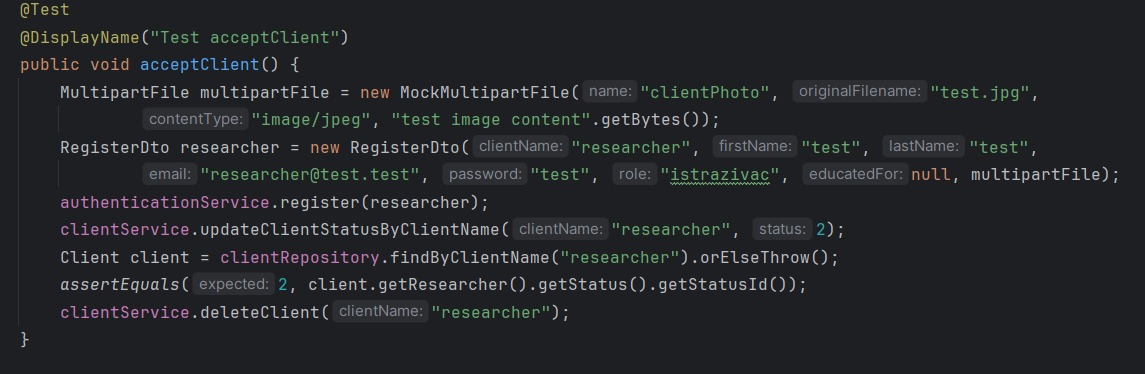
\includegraphics[width=\textwidth]{slike/istrazivac1.JPEG}
				\caption{Testiranje prihvaćanja istraživača }
				\label{fig:dijagram_baze}
			\end{figure}
			
			\begin{figure}[H]
				\centering
				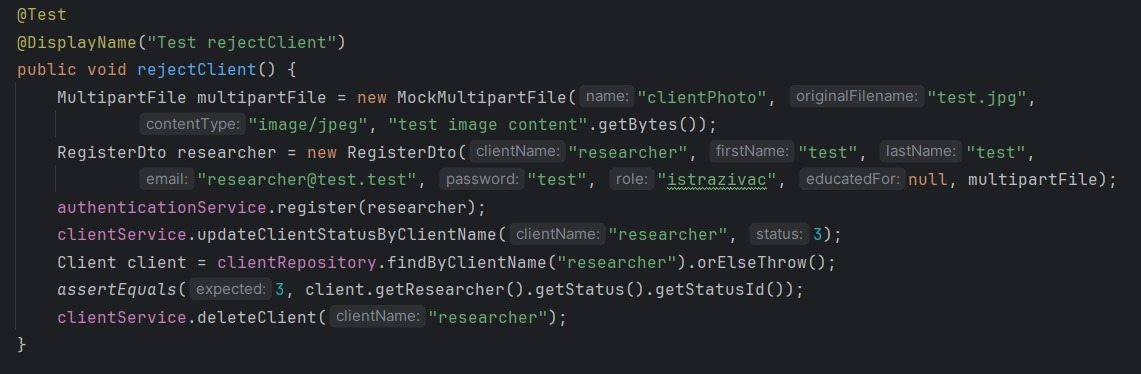
\includegraphics[width=\textwidth]{slike/istrazivac2.JPEG}
				\caption{Testiranje odbijanja istraživača }
				\label{fig:dijagram_baze}
			\end{figure}
			
			Ovaj test provjerava postoji li uopće admin u bazi. Test koda prikazan je na slici 5.8.
			
			\begin{figure}[H]
				\centering
				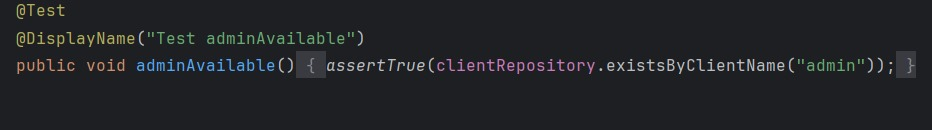
\includegraphics[width=\textwidth]{slike/admin1.JPEG}
				\caption{Testiranje postoji li admin u bazi}
				\label{fig:dijagram_baze}
			\end{figure}
			
			Na slici 5.9 prikazana je snimka zaslona terminala u IntelliJ IDE-u, kao rezultat izvodenja prethodno navedenih osam ispitnih slučajeva. 
			
			\begin{figure}[H]
				\centering
				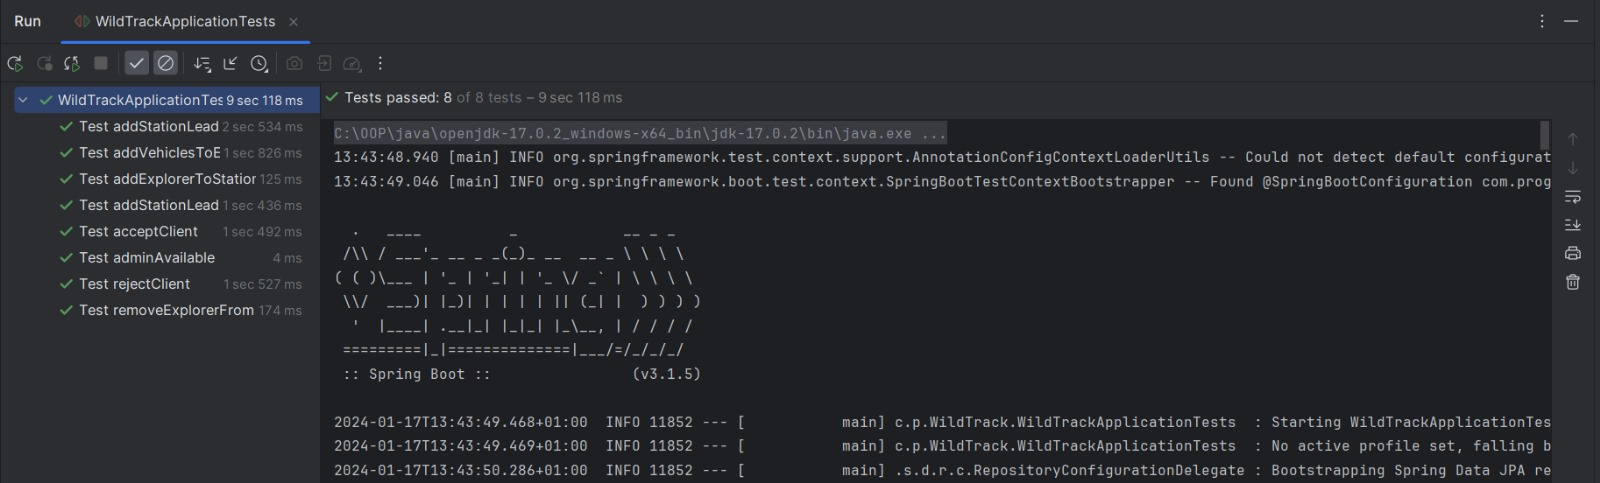
\includegraphics[width=\textwidth]{slike/ispis.JPEG}
				\caption{Rezultati ispitivanja pomoću Spring-a i JUnit-a}
				\label{fig:dijagram_baze}
			\end{figure}
			
			\vspace{108pt}
			
			\subsection{Ispitivanje sustava}
			
			 Ispitivanje sustava provedeno je pomoću dodatka za preglednik Selenium IDE. U nastavku su opisani provedeni ispitni slučajevi. Na slici 5.10 vidimo kako se admin pokušava ulogirati sa korisničkim imenom "admin2". To je pogrešno korisničko ime te se admin neće moći prijaviti. Slika 5.12 prikazuje isto to samo admin se prijavljuje pomoću korisničkog imena "admin" koje je njegovo pravo i uspješno se prijavljuje u aplikaciju.
			 
			 \begin{figure}[H]
			 	\centering
			 	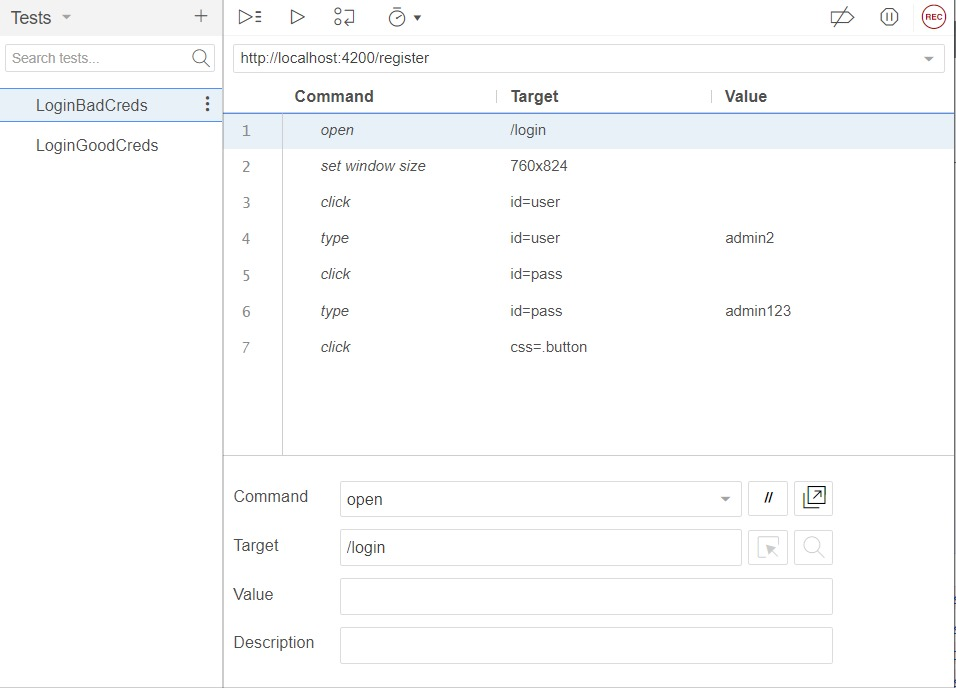
\includegraphics[width=\textwidth]{slike/krivi.JPEG}
			 	\caption{Parametri sa pogrešnim korisničkim imenom}
			 	\label{fig:dijagram_baze}
			 \end{figure}
			 
			 \begin{figure}[H]
			 	\centering
			 	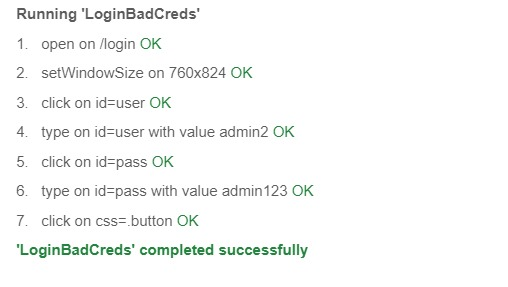
\includegraphics[width=\textwidth]{slike/krivi2.JPEG}
			 	\caption{Rezultat prvog ispitnog slučaja}
			 	\label{fig:dijagram_baze}
			 \end{figure}
			 
			 \begin{figure}[H]
			 	\centering
			 	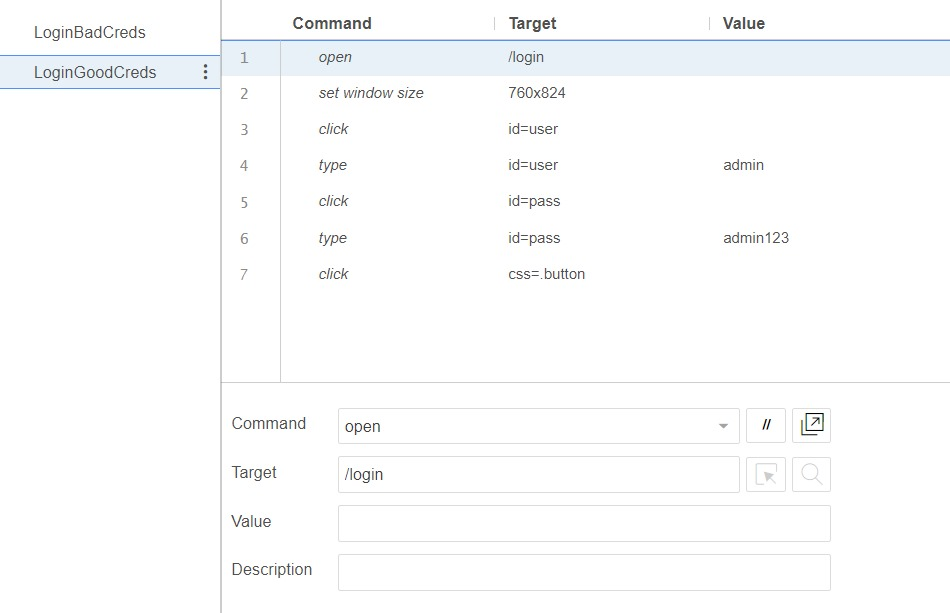
\includegraphics[width=\textwidth]{slike/pravi.JPEG}
			 	\caption{Parametri sa valjanim korisničkim imenom}
			 	\label{fig:dijagram_baze}
			 \end{figure}
		
			  \begin{figure}[H]
			 	\centering
			 	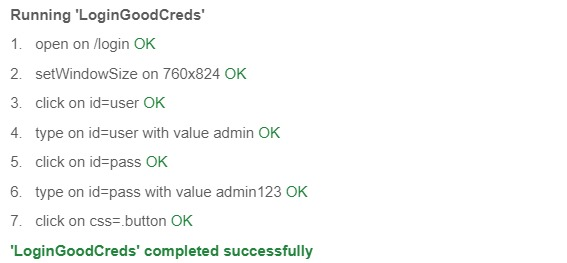
\includegraphics[width=\textwidth]{slike/pravi2.JPEG}
			 	\caption{Rezultat drugog ispitnog slučaja}
			 	\label{fig:dijagram_baze}
			 \end{figure}
			 
		\vspace{324pt}	 
		\section{Dijagram razmještaja}
			
			Na slici 5.14 nalazi se dijagram razmještaja. Dijagram razmještaja prikazuje fizičku strukturu programskog sustava. Glavna svrha mu je pobliže prikazati arhitekturu razmještaja sustava. Korisnici pristupaju aplikaciji korištenjem web preglednika. Komunikacija se odvija putem protokola HTTP. Na platformi Render se nalaze poslužitelji za frontend, backend i bazu podataka.
			
			\begin{figure}[H]
				\centering
				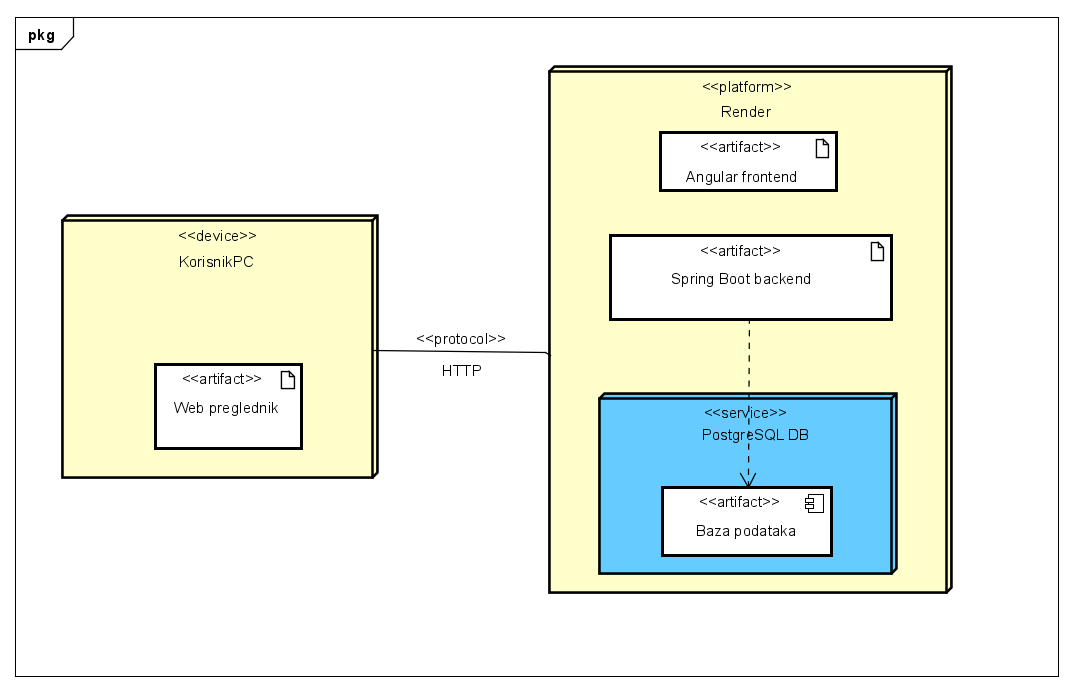
\includegraphics[width=\textwidth]{slike/Dijagram_razmjestaja.PNG}
				\caption{Dijagram razmještaja }
				\label{fig:dijagram_baze}
			\end{figure}
			
		\vspace{108pt}
		
		
		\section{Upute za puštanje u pogon}
		
			Pri puštanju u pogon prvo je potrebno registrirati se na stranici "Render". Preporučamo koristeći vlastiti GitHub profil. Preduvjet za puštanje web aplikacije u pogon je zasebno pustiti u pogon backend, frontend i postgreSQL bazu podataka. Za deploy baze podataka odabiremo opciju "New" $\rightarrow$  "PostgreSQL". Nakon toga potrebno je upisati ime baze i odabrati instancu. U našem slučaju ta instanca je "free". Zatim kreiramo bazu. Postupak kako to učiniti prikazan je na slikama 5.15 i 5.16. 
			
		
			
			\begin{figure}[H]
				\centering
				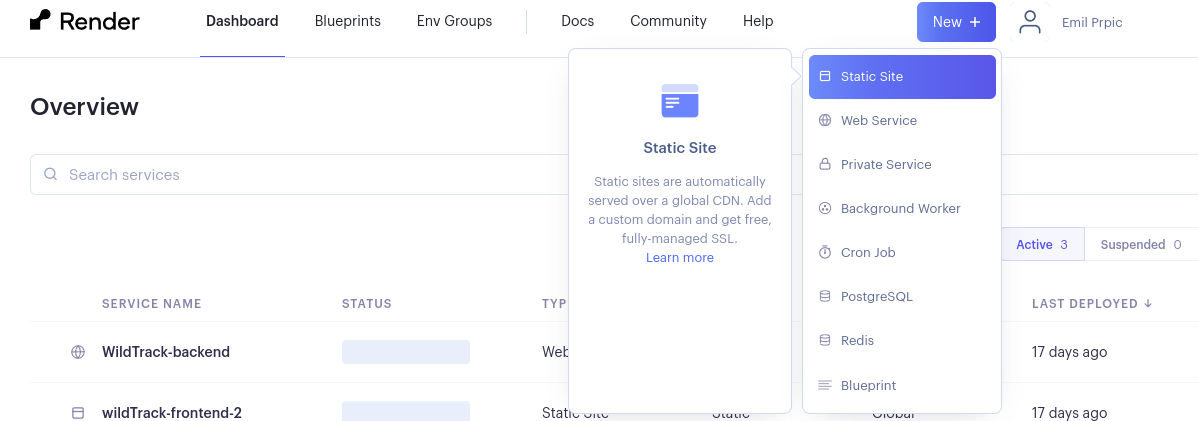
\includegraphics[width=\textwidth]{slike/slika1.PNG}
				\caption{Puštanje u pogon baze }
				\label{fig:dijagram_baze}
			\end{figure}
			
			\begin{figure}[H]
				\centering
				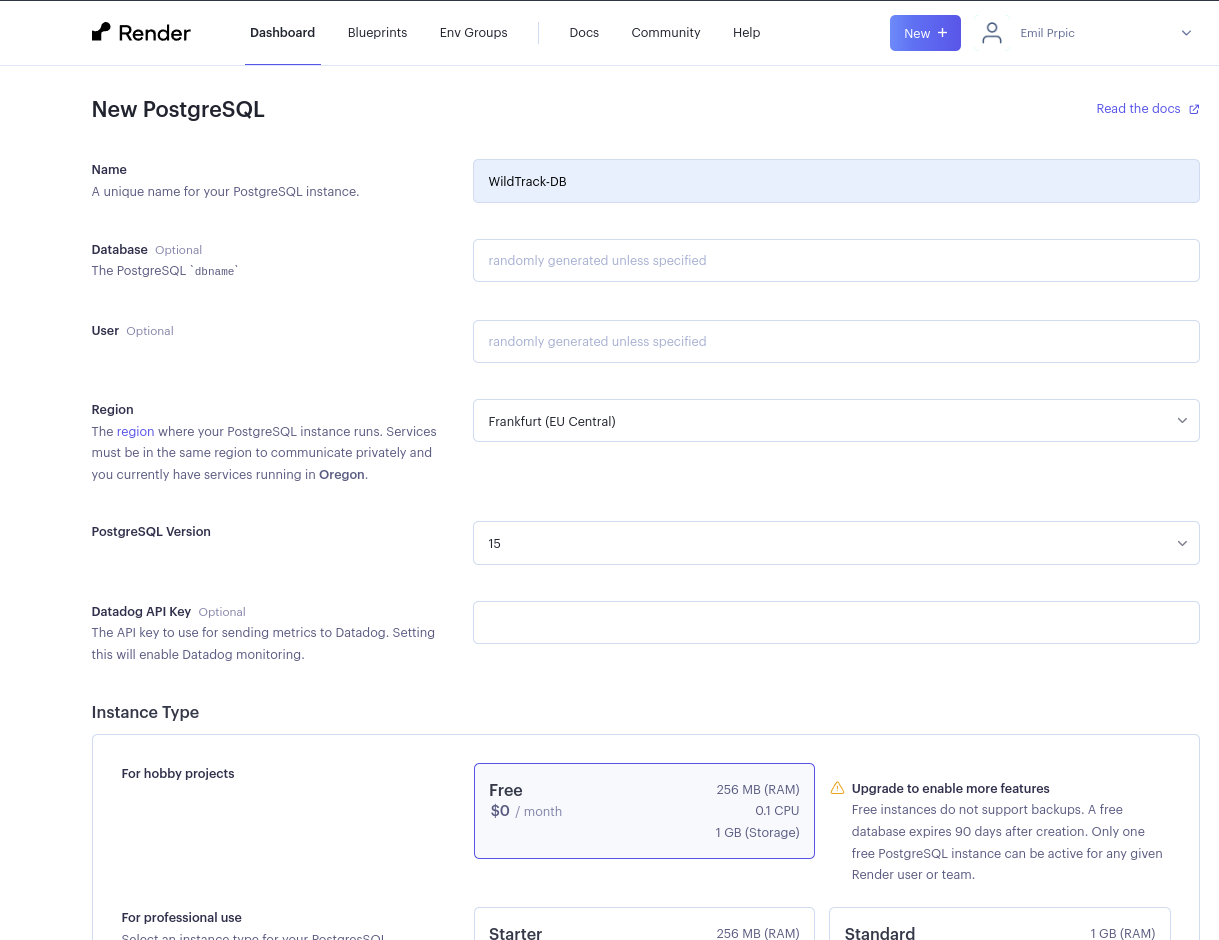
\includegraphics[width=0.7\textwidth]{slike/slika2.PNG}
				\caption{Puštanje u pogon baze}
				\label{fig:dijagram_baze}
			\end{figure}
			
			
			Sljedeće ćemo pustiti u pogon backend. Odabiremo opciju "New" $\rightarrow$ "Web Service" $\rightarrow$ "Build and deploy from Git repo $\rightarrow$ povežete GitHub profil i odaberete projekt koji želite pustiti u pogon. Postavite ime, regiju i root direktorij. Mi koristimo takozvani "monorepo" pa u root upisujemo "IzvorniKod/BackEnd". Postupak kako pustiti u pogon backend vidljiv je na sljedećim slikama.
			
			\begin{figure}[H]
				\centering
				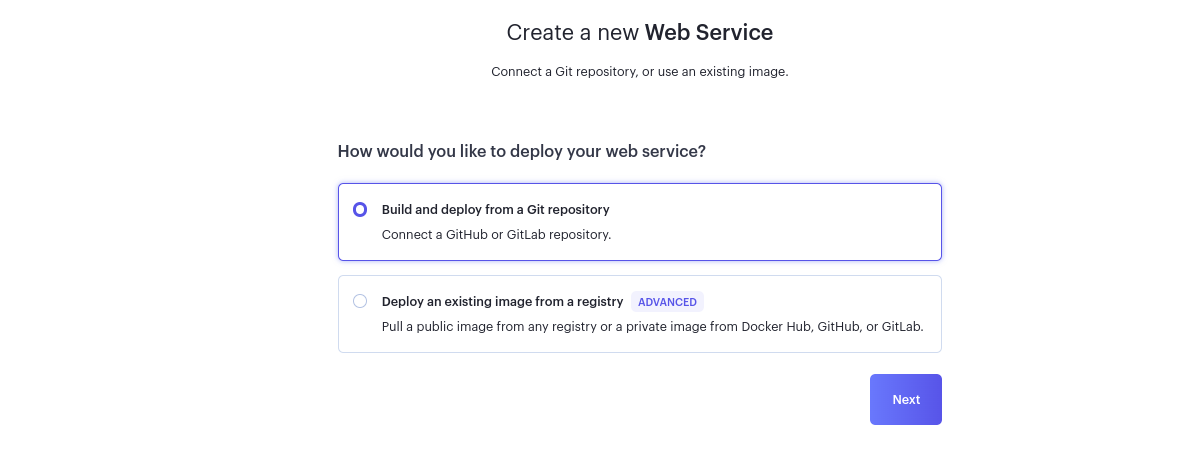
\includegraphics[width=\textwidth]{slike/slika3.PNG}
				\caption{Puštanje u pogon backenda }
				\label{fig:dijagram_baze}
			\end{figure}
			
			\begin{figure}[H]
				\centering
				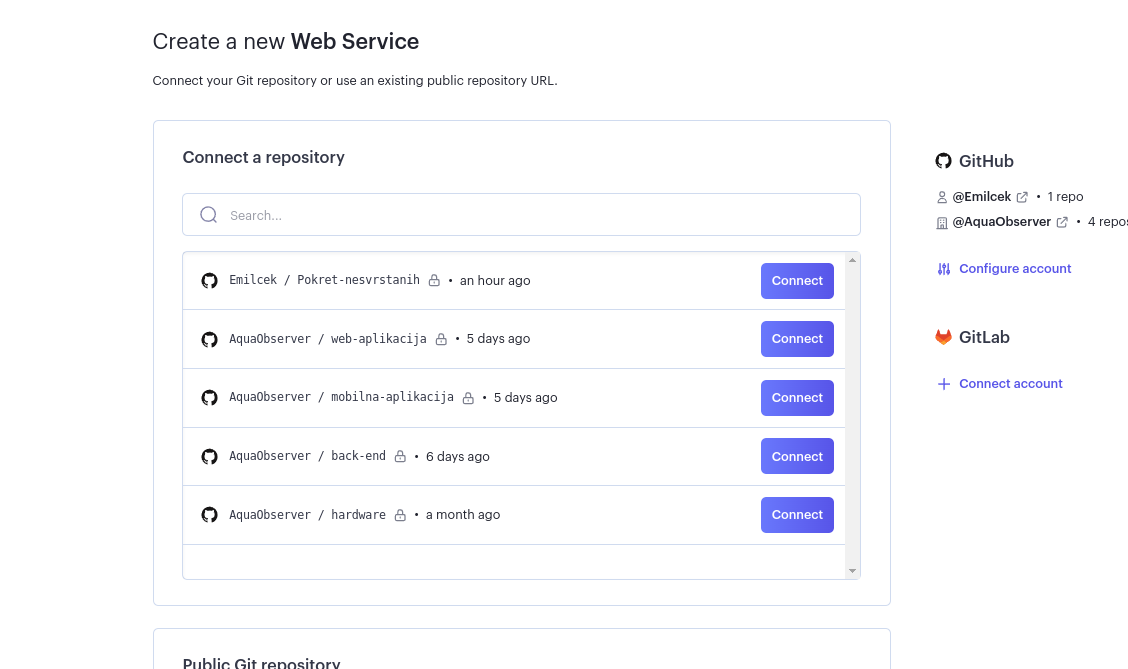
\includegraphics[width=\textwidth]{slike/slika4.PNG}
				\caption{Povezivanje s GitHub profilom }
				\label{fig:dijagram_baze}
			\end{figure}
			
			\begin{figure}[H]
				\centering
				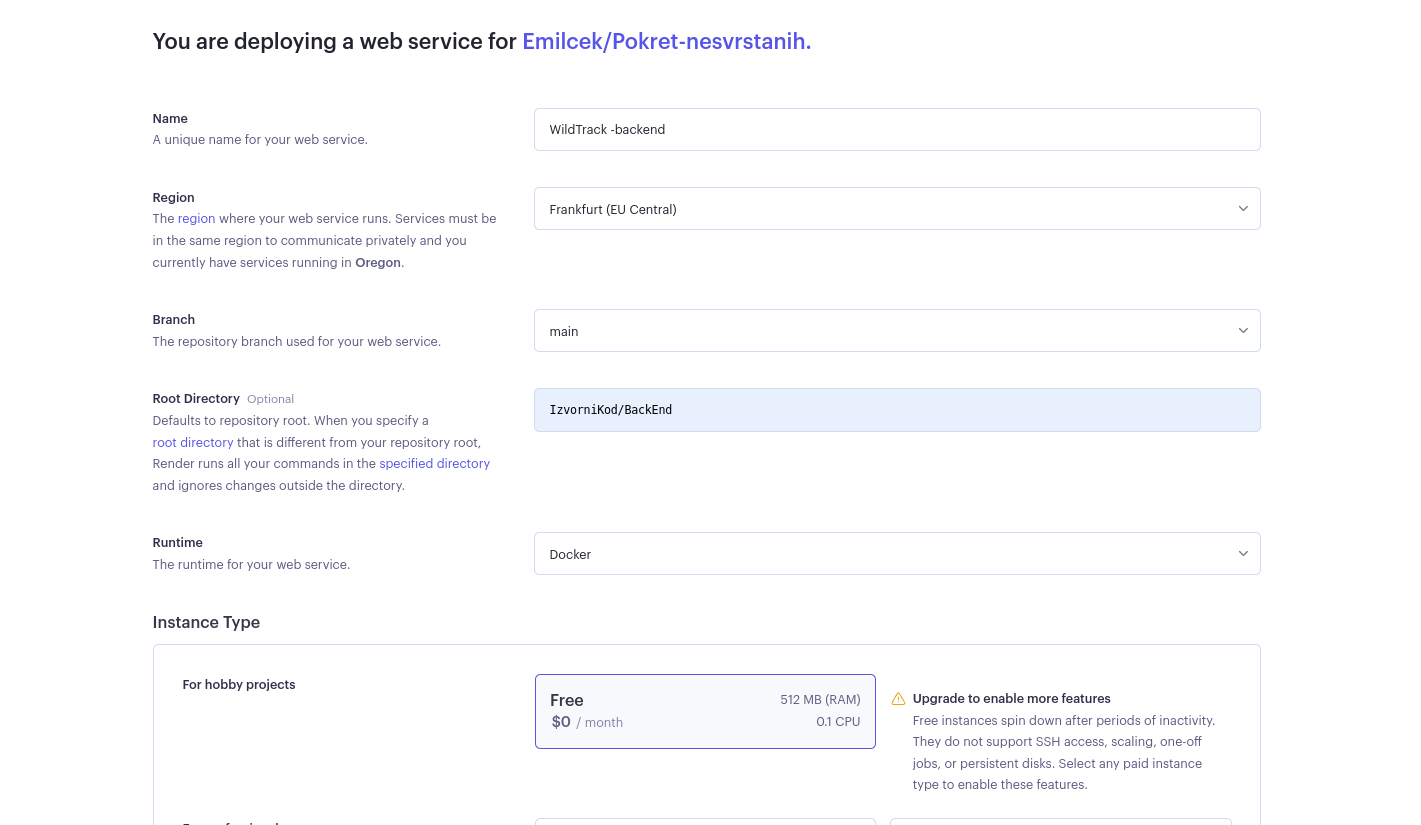
\includegraphics[width=\textwidth]{slike/slika5.PNG}
				\caption{Postavljanje imena, regije i root direktorija}
				\label{fig:dijagram_baze}
			\end{figure}
		
			Puštanje u pogon frontenda je vrlo slično. Odaberemo opciju "New" $\rightarrow$ "Static site" $\rightarrow$ odabir projekta $\rightarrow$ postavke konfiguracije možete vidjeti na slici 5.20.
			
			\begin{figure}[H]
				\centering
				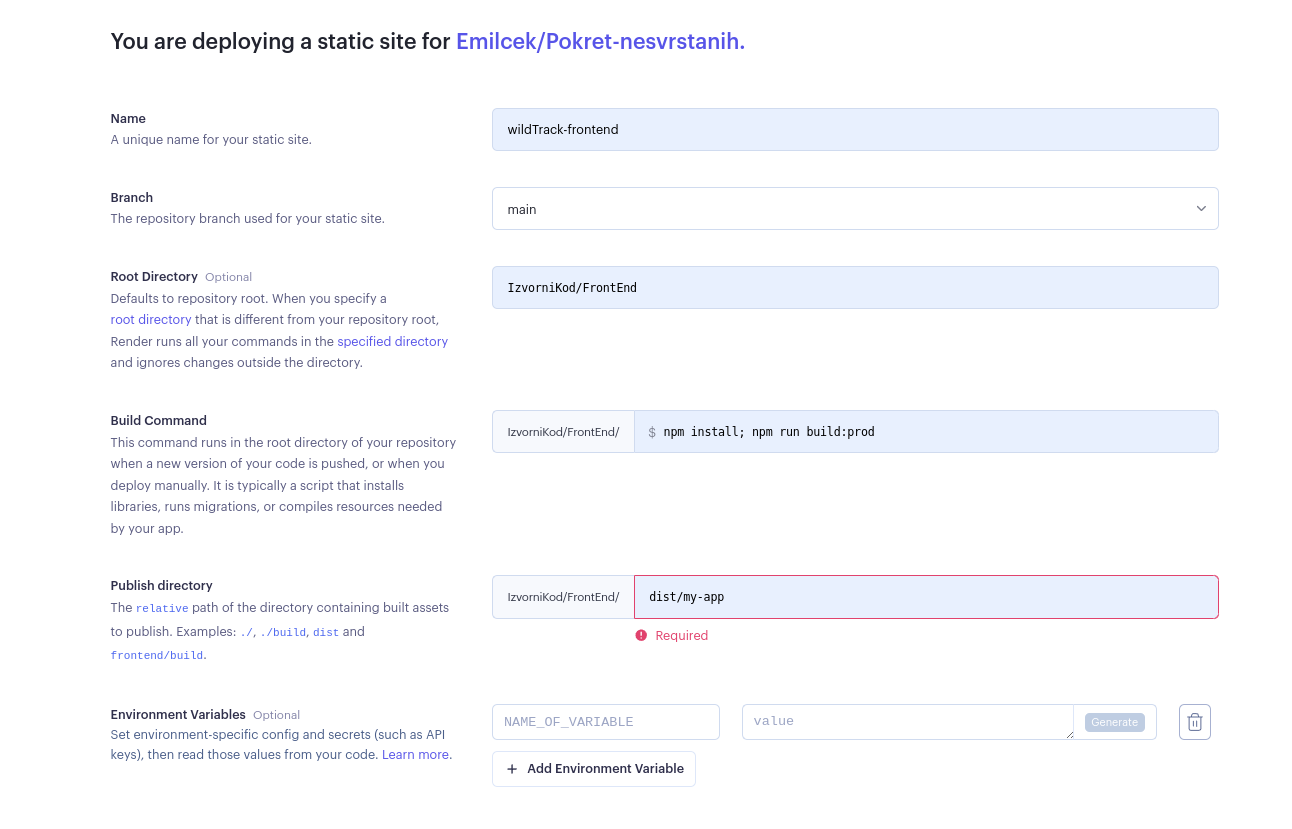
\includegraphics[width=0.7\textwidth]{slike/slika6.PNG}
				\caption{Postavke konfiguracije za frontend}
				\label{fig:dijagram_baze}
			\end{figure}
			
			\vspace{72pt}
			Sljedeći vrlo važan korak je postavljanje environment varijabli na frontend i backend. Kako to izgleda prikazano je na slikama 5.21 i 5.22.
			
			\begin{figure}[H]
				\centering
				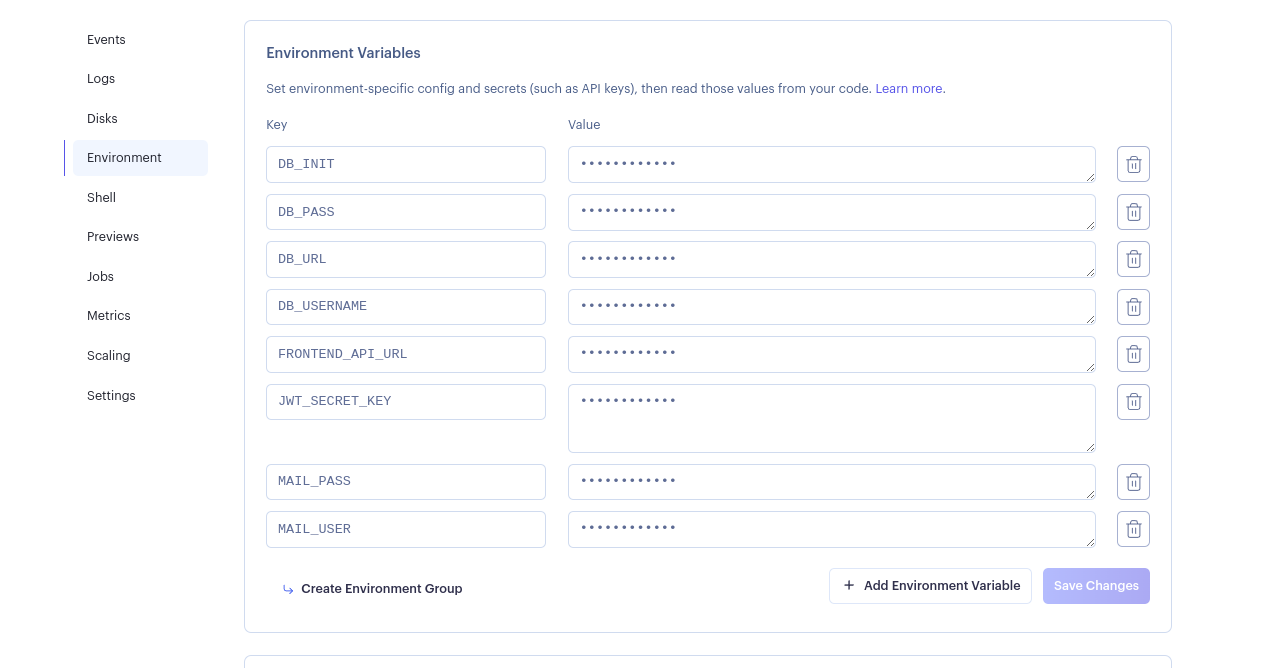
\includegraphics[width=\textwidth]{slike/slika7.PNG}
				\caption{Postavljanje environment varijabli za backend}
				\label{fig:dijagram_baze}
			\end{figure}
			
			\begin{figure}[H]
				\centering
				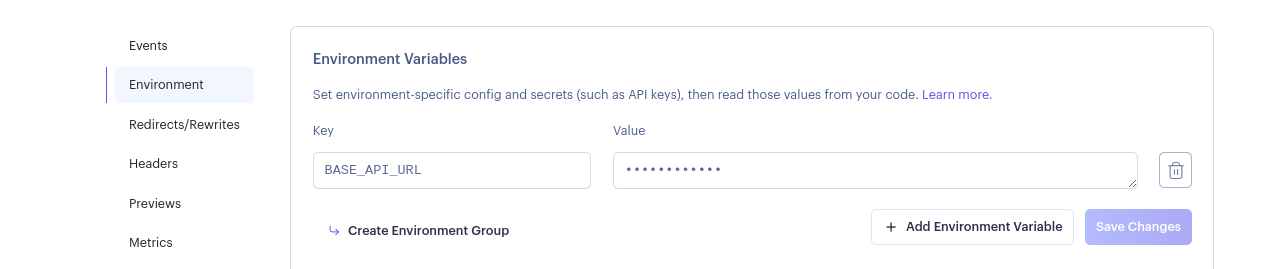
\includegraphics[width=\textwidth]{slike/slika8.PNG}
				\caption{Postavljanje environment varijabli za frontend}
				\label{fig:dijagram_baze}
			\end{figure}
			
			
			Kako bi ste došli do varijabli koje su vezane uz bazu na dashbordu odaberete bazu i unutar connections se nalaze sve slike, a API URL za frontend odnosno backend se nađe tako da se odabere frontend ili backend slika.
			
			\begin{figure}[H]
				\centering
				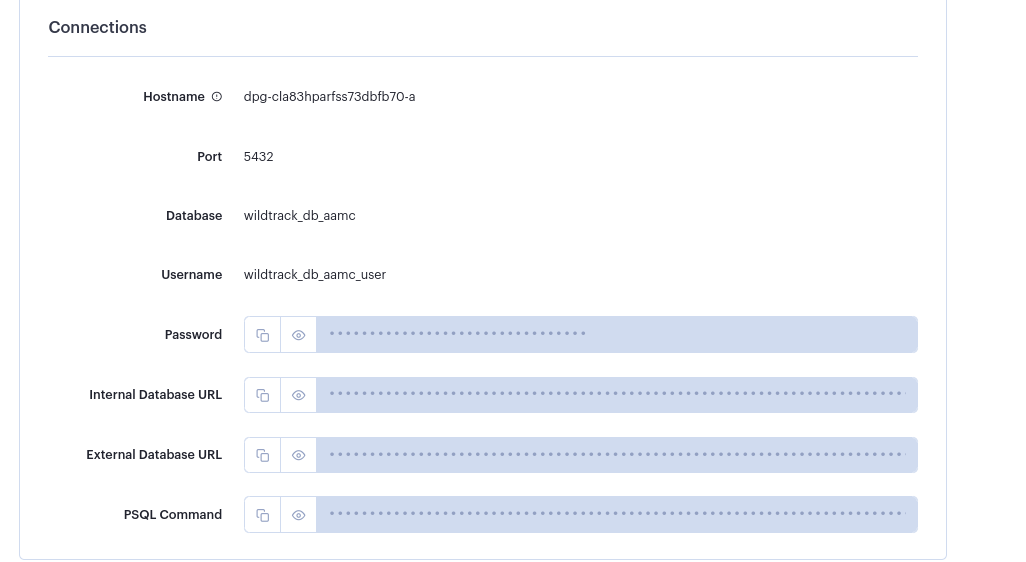
\includegraphics[width=\textwidth]{slike/slika9.PNG}
				\caption{Prikaz connections-a}
				\label{fig:dijagram_baze}
			\end{figure}
			
			\begin{figure}[H]
				\centering
				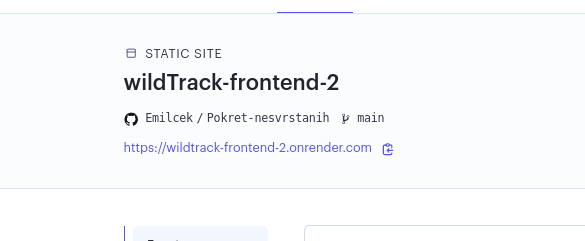
\includegraphics[width=\textwidth]{slike/slika10.PNG}
				\caption{API URL za frontend/backend}
				\label{fig:dijagram_baze}
			\end{figure}
		
		